\chapter{Buck-boost equations}\label{ch:Appbuckboost}

The way the buck-boost converter works has been discussed in the introductory chapter \ref{N_INV_BB} The equations that can be used for this type of converter depends on, in which mode the converter are working in. When working in the buck mode the equations below will be used when we see the converter as ideal. 

\section{Buck mode}

The voltages and currents in the different switch stages can be seen in figure \ref{CCM_buck}

\begin{figure}[htbp]
	\begin{center}
		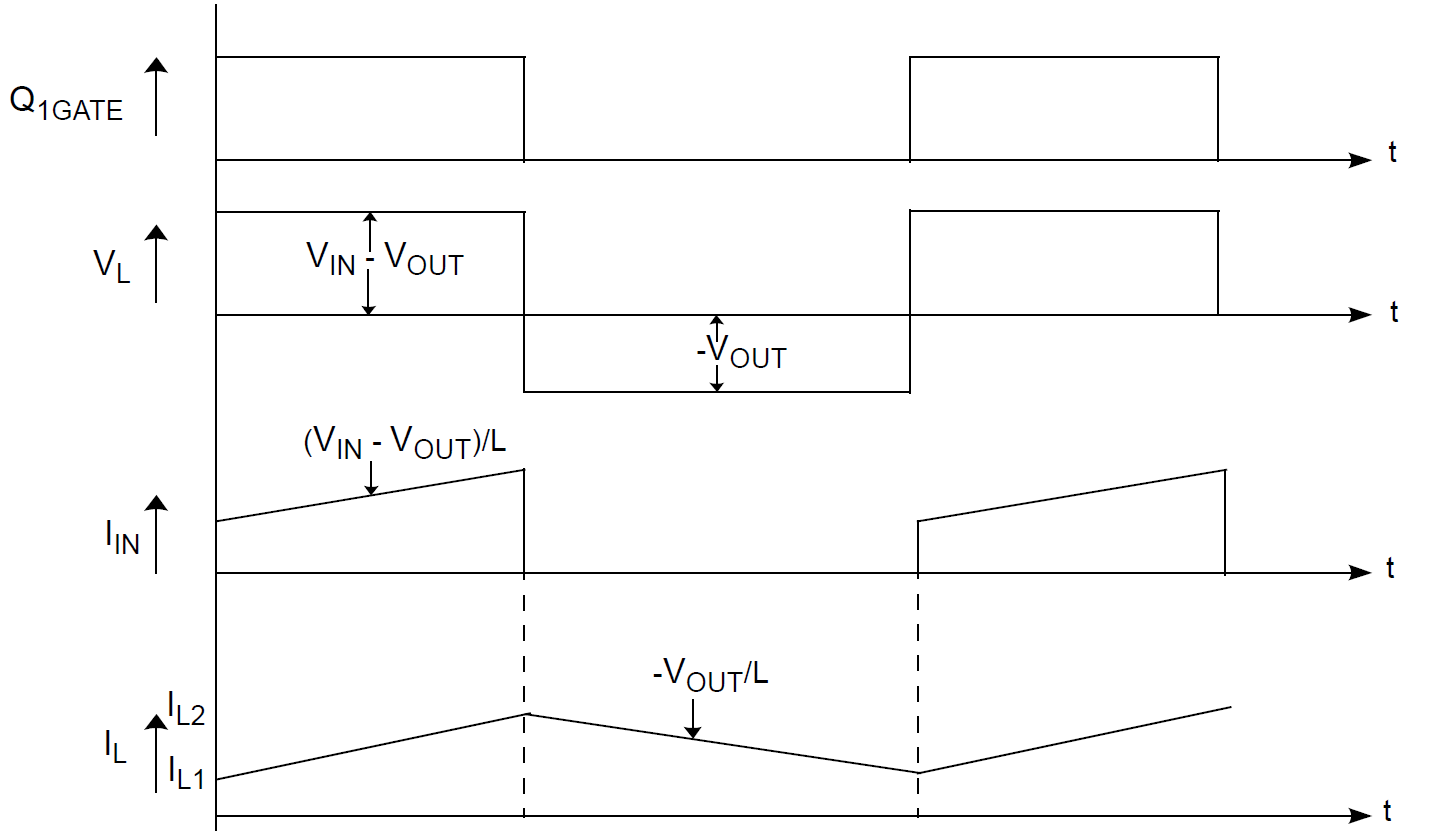
\includegraphics[width=0.6\textwidth]{../Pictures/P1/Appendix/buck_currents}
		\caption{Ideal buck converter in CCM \cite{CCM_buck}.}
		\label{CCM_buck}
	\end{center}	
\end{figure}

Working in CCM mode means that the current through the inductor never falls to zero. When the switch is on(closed) the voltage across the inductor will be: 

\begin{equation}
V_L = V_{in}-V_{out}
\end{equation} 

The current through the inductor rises linearly and no current will flow through the diode.
When the switch is off(open) the diode will be forward biased which means the voltage across the inductor will be:

\begin{equation}
V_L = -V_{out}
\end{equation} 

As seen in the figure \ref{CCM_buck} the current will decrease in this state, until the switch turns on again.

This equations show that energy will be stored in the inductor during the on time and decreases in the off time. This means that the inductor is used to transfer the energy from the input to the output of the converter. 
When working in a steady state operation the transfer function of the buck converter is:

\begin{equation}
V_{out} = D\cdot V_{in}
\end{equation}

\noindent The current seen at the output will be the average current in the inductor:

\begin{equation} \label{Iavg}
I_{out}=I_{Lavg}
\end{equation}

The inductance can be calculated by using the switching frequency and wanted current ripple in the inductor:

\begin{equation}\label{buckind}
L = \frac{V_{in}\cdot D(1-D)}{\Delta I_L \cdot f_s}
\end{equation}

\noindent That equation will be used to calculate the peak current in the inductor:

\begin{equation}
I_{L,peak} = I_{out} + \frac{\Delta I_{L}}{2}
\end{equation}

There are several factors that contribute to the output voltage ripple. Basically the output voltage will rise and fall when the capacitor is charging and discharging. It can be found by calculating $\Delta V_{out} = \frac{\Delta Q}{C}$, where $\Delta Q$ is the amount of charge. This value is found by integrating $I_L$ from $t_1$ to $t_2$. By doing that $\Delta Q = \frac{\Delta I_L}{8}\cdot f_s$. where $\Delta I_L = (V_{out}\cdot t_2)/L$ Which means the output voltage ripple can be calculated with \cite{buck_equation}:
 
\begin{equation} \label{buckc} 
C_{out} = \frac{V_{in}\cdot (1-D)}{8\cdot \Delta V_{out}\cdot f_s^2\cdot L}  
\end{equation}     

For the input capacitor the capacitance can be calculated with the equation below \cite{underthehood}:
\begin{equation}
\label{buckcin}
C_{in} = \frac{I_{out}\cdot D\cdot (1-D)}{\Delta V_{out}\cdot f_s}
\end{equation}   

\section{Boost mode}
When working in boost mode the output voltage will be larger than the input voltage. The voltages and currents in the different switch stages can be seen in figure \ref{CCM_boost}. \todo{update figure refs when stef is done, NHF}

\begin{figure}[H]
	\begin{center}
		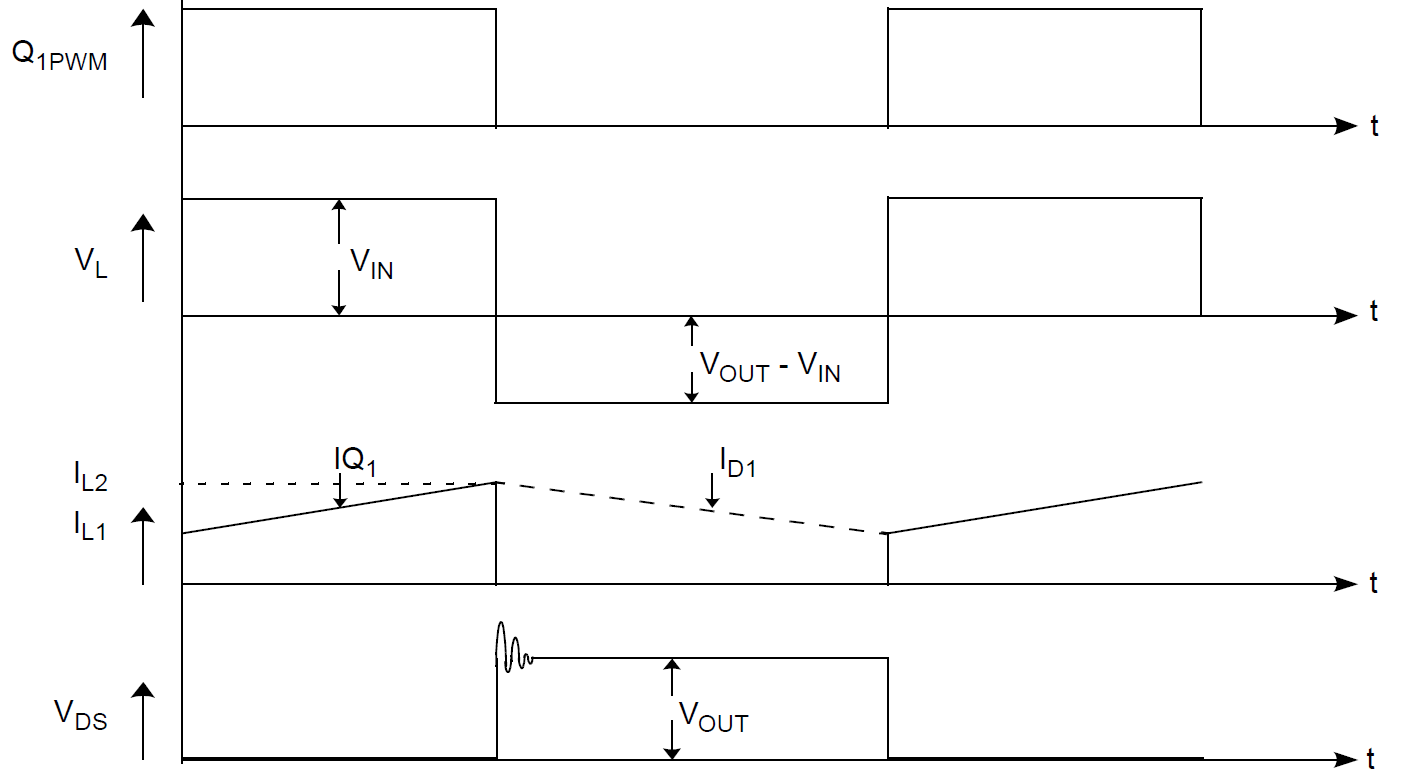
\includegraphics[width=0.6\textwidth]{../Pictures/P1/Appendix/boost_currents}
		\caption{Ideal boost converter in CCM \cite{CCM_boost}.}
		\label{CCM_boost}
	\end{center}	
\end{figure}
In the boost mode CCM will still be used. When the switch is on the voltage across the inductor will be:

\begin{equation}
V_L = V_{in}
\end{equation}

In this state the inductor current will increase. On the other hand in the off-state the inductor will transfer its energy to the capacitor. Here the voltage across the inductor will be:

\begin{equation}
V_L = V_{in}-V_{out}
\end{equation}

In figure \ref{CCM_boost} it can be seen that we are working in CCM because the current never reaches zero. 
When working in steady state the increase of energy stored in the inductor must be equal to the energy transfered to the capacitor during the off state. This means that $\Delta I_{Lon}+\Delta I_{Loff}$. Integrating and reducing these expressions will lead to:

\begin{equation}
V_{out} = \frac{1}{1-D}\cdot V_{in}
\end{equation}
 
\noindent The average current through the inductor will be calculated as below:
\begin{equation}
I_{Lavg} = \frac{1}{1-D}\cdot I_{out}
\end{equation}

\noindent The needed inductance can be calculated using the switching frequency and the wanted current ripple in the inductor:

\begin{equation}\label{boostind}
L = \frac{V_{in}\cdot D}{\Delta I_L \cdot f_s}
\end{equation}

\noindent The peak current through the inductor can be found like this:

\begin{equation}
I_{Lmax} = \frac{1}{1-D}\cdot I_{out}+\frac{\Delta I_{Lmax}}{2}
\end{equation}

\noindent The output voltage ripple can be calculated with equation \ref{boostc}\cite{boost_equation}:

\begin{equation}\label{boostc}
\Delta V_{out} = \frac{D\cdot I_{out}}{f_s \cdot C_{out}}
\end{equation} 

\noindent The input capacitor value can be found with equation \ref{boostcin}\cite{underthehood}:

\begin{equation} \label{boostcin}
C_{in} = \frac{I_{out}\cdot D\cdot (1-D)}{\Delta V_{out} \cdot f_s}
\end{equation}  
